\section{Implementasi dan Pengujian}

\subsection{Pseudocode untuk Alternatif Solusi}

\subsubsection{mainbot}

\begin{pseudocode}{BaseRobot.java}
    function moveTo(target: Location) -> boolean
    { Menentukan langkah pergerakan terbaik menuju target dengan penalti trail }

    { Deklarasi }
    C : himpunan_kandidat_arah
    dir, bestDir : Direction
    score, bestScore, trailPenalty : integer
    nextLoc : Location

    { Algoritma }
    if not isMovementReady() then return false end if
    
    bestScore <- 999999 { Mencari nilai minimum (jarak terpendek) }
    bestDir <- null
    C <- {NORTH, NORTHEAST, EAST, SOUTHEAST, SOUTH, SOUTHWEST, WEST, NORTHWEST}

    while C != {} do
        dir <- SELEKSI(C)
        C <- C - {dir}
        
        if canMove(dir) then
            nextLoc <- getCurrentLocation() + dir
            
            { Fungsi Seleksi: Jarak Euclidean + Penalti Riwayat (Trail) }
            trailPenalty <- getTrailPenalty(nextLoc)
            score <- distanceSquared(nextLoc, target) + trailPenalty
            
            { Keputusan Greedy: Pilih skor terendah }
            if score < bestScore then
                bestScore <- score
                bestDir <- dir
            end if
        end if
    end while

    if bestDir != null then
        move(bestDir)
        recordTrail(getCurrentLocation())
        return true
    end if
    return false
\end{pseudocode}

\begin{pseudocode}{TowerUnit.java}
    function decideSpawnType(totalUnits: integer) -> UnitType
    { Memilih unit yang akan diproduksi berdasarkan rasio populasi saat ini }

    { Deklarasi }
    rSoldier, rSplasher, rMopper : float

    { Algoritma }
    if totalUnits = 0 then return SOLDIER end if

    { Hitung Rasio Distribusi Pasukan }
    rSoldier <- getSoldierCount() / totalUnits
    rSplasher <- getSplasherCount() / totalUnits
    rMopper <- getMopperCount() / totalUnits

    { Fungsi Seleksi Greedy: Prioritaskan rasio terendah yang belum terpenuhi }
    if rMopper < 0.15 then
        return MOPPER
    else if rSoldier < 0.40 then
        return SOLDIER
    else if rSplasher < 0.45 then
        return SPLASHER
    else
        return SOLDIER { Default fallback }
    end if
\end{pseudocode}

\begin{pseudocode}{SplasherUnit.java}
    function findDensityTarget() -> Location
    { Menentukan target koordinat pergerakan menuju kuadran dengan densitas cat tertinggi }

    { Deklarasi }
    C : himpunan_kandidat_tile
    quadScore : array[0..3] of integer
    quadCount : array[0..3] of integer
    bestQ : integer
    maxDensity, currentDensity : float

    { Algoritma }
    C <- getAllVisibleTiles()
    
    while C != {} do
        tile <- SELEKSI(C)
        C <- C - {tile}
        q <- getQuadrantIndex(tile.location)
        
        quadCount[q] <- quadCount[q] + 1
        if not isAlly(tile.paint) then
            { Bobot Greedy: Musuh = 3, Kosong = 1 }
            quadScore[q] <- quadScore[q] + (isEnemy(tile.paint) ? 3 : 1)
        end if
    end while

    { Cari Kuadran dengan Densitas Keuntungan Maksimal }
    maxDensity <- -1.0
    for i <- 0 to 3 do
        currentDensity <- quadScore[i] / quadCount[i]
        if currentDensity > maxDensity then
            maxDensity <- currentDensity
            bestQ <- i
        end if
    end for

    return getCoordinateFromQuadrant(bestQ)
\end{pseudocode}

\begin{pseudocode}{MopperUnit.java}
    procedure doMobCombat()
    { Memilih arah ayunan mop swing secara greedy untuk mengenai musuh sebanyak mungkin }

    { Deklarasi }
    C : himpunan_kandidat_arah
    dir, bestDir : Direction
    hits, bestHits : integer

    { Algoritma }
    if not isActionReady() then stop end if

    bestHits <- 0
    bestDir <- null
    C <- {NORTH, NORTHEAST, EAST, SOUTHEAST, SOUTH, SOUTHWEST, WEST, NORTHWEST}

    while C != {} do
        dir <- SELEKSI(C)
        C <- C - {dir}

        if canMopSwing(dir) then
            { Fungsi Seleksi: Hitung jumlah robot musuh dalam jangkauan ayunan 3-tile }
            hits <- countMopSwingHits(dir)

            if hits > bestHits then
                bestHits <- hits
                bestDir <- dir
            end if
        end if
    end while

    { Eksekusi Aksi }
    if bestDir != null then
        mopSwing(bestDir)
    end if
\end{pseudocode}

\begin{pseudocode}{SoldierUnit.java}
    procedure doInitialPaint(homeTower: Location)
    { Pembagian area kerja Greedy di sekitar menara awal secara simetris }

    { Deklarasi }
    C : himpunan_kandidat_tile
    tile : MapInfo
    tLoc : Location
    isRoleA : boolean

    { Algoritma }
    isRoleA <- (getID() mod 2 = 0)
    C <- getNearbyMapInfos(homeTower, 8)

    while C != {} do
        tile <- SELEKSI(C)
        C <- C - {tile}
        tLoc <- tile.location

        { Fungsi Kelayakan Berdasarkan Peran }
        if isRoleA then
            if not (tLoc.x < homeTower.x or (tLoc.x = homeTower.x and tLoc.y < homeTower.y)) then 
                continue 
            end if
        else
            if (tLoc.x < homeTower.x or (tLoc.x = homeTower.x and tLoc.y < homeTower.y)) then 
                continue 
            end if
        end if

        { Aksi Greedy Pengecatan }
        if not isAlly(tile.paint) and canAttack(tLoc) then
            if isActionReady() then
                attack(tLoc)
                stop { Keluar dari prosedur setelah aksi berhasil }
            end if
        end if
    end while
\end{pseudocode}

\subsubsection{altbot1}
\begin{pseudocode}{Navigation.java}
    function moveGreedyMacro(targetDir: Direction, history: array of Location, isSplasher: boolean) -> boolean
    { Mencari dan mengeksekusi arah pergerakan terbaik berdasarkan nilai heuristik tertinggi }

    { Deklarasi }
    C : himpunan_kandidat_arah
    dir, bestDir : Direction
    score, bestScore : integer
    myLoc, nextLoc, center : Location

    { Algoritma }
    bestScore <- -99999
    bestDir <- null
    myLoc <- getCurrentLocation()
    center <- getCenterLocation()

    { Inisialisasi himpunan kandidat dengan 8 arah mata angin }
    C <- {NORTH, NORTHEAST, EAST, SOUTHEAST, SOUTH, SOUTHWEST, WEST, NORTHWEST}

    while C != {} do
        dir <- SELEKSI(C) { Pilih satu arah dari himpunan kandidat }
        C <- C - {dir}
        
        if canMove(dir) then
            nextLoc <- myLoc + dir
            score <- 0
            
            { Fungsi Obyektif: Hitung bobot keuntungan dari arah ini }
            score <- score + evaluateDirectionAlignment(dir, targetDir)
            
            if getPaint(nextLoc) = ALLY then
                score <- score + 8
            else if getPaint(nextLoc) = EMPTY then
                score <- score + 10
            else
                score <- score - 15
            end if
            
            if distance(nextLoc, center) < distance(myLoc, center) then
                score <- score + 5
            end if
            
            { Fungsi Kelayakan / Penalti }
            score <- score - evaluateTowerStarvation(nextLoc)
            score <- score - evaluateHistoryPenalty(nextLoc, history)
            
            { Pembaruan solusi optimum lokal }
            if score > bestScore then
                bestScore <- score
                bestDir <- dir
            end if
        end if
    end while

    if bestDir != null then
        move(bestDir)
        return true
    else
        return false
    end if
\end{pseudocode}

\begin{pseudocode}{Heuristic.java}
    function pickBestTarget(enemies: array of Robot, myLoc: Location) -> Robot
    { Mencari target musuh dengan ancaman tertinggi dan jarak terdekat }

    { Deklarasi }
    C : himpunan_kandidat_musuh
    enemy, bestTarget : Robot
    score, bestScore, dist, bestDist : integer

    { Algoritma }
    C <- enemies { Kandidat adalah semua musuh yang terdeteksi sensor }
    bestTarget <- null
    bestScore <- -99999
    bestDist <- 99999

    while C != {} do
        enemy <- SELEKSI(C)
        C <- C - {enemy}
        
        { Fungsi Obyektif }
        score <- scoreAttackTarget(enemy)
        dist <- distance(myLoc, enemy.location)
        
        { Keputusan Greedy: Ambil yang skornya paling besar, atau jika sama besar ambil yang terdekat }
        if (score > bestScore) or ((score = bestScore) and (dist < bestDist)) then
            bestScore <- score
            bestDist <- dist
            bestTarget <- enemy
        end if
    end while

    return bestTarget
\end{pseudocode}

\begin{pseudocode}{Heuristic.java}
    function scoreTowerType(ruinLoc: Location, currentChips: integer, currentPaint: integer, round: integer) -> TowerType
    { Menentukan tipe menara berdasarkan kondisi sumber daya yang paling kritis saat ini }

    { Deklarasi }
    isFrontline : boolean
    paintTowersCount, moneyTowersCount : integer

    { Algoritma }
    isFrontline <- checkEnemyPaintNearby(ruinLoc, 16)

    { Evaluasi Greedy: Selesaikan masalah yang paling mendesak terlebih dahulu }
    if (currentPaint < 1000) or (round <= 100) then
        return PAINT_TOWER
    end if

    if isFrontline and (currentChips >= 2000) and (currentPaint >= 1000) then
        return DEFENSE_TOWER
    end if

    paintTowersCount <- countTowers(PAINT_TOWER)
    moneyTowersCount <- countTowers(MONEY_TOWER)

    { Penyeimbangan Rasio Greedy }
    if moneyTowersCount = 0 then
        return MONEY_TOWER
    end if

    if (paintTowersCount / moneyTowersCount) < 2.0 then
        return PAINT_TOWER
    else
        return MONEY_TOWER
    end if
\end{pseudocode}

\begin{pseudocode}{Splasher.java}
    function findUnpaintedCluster(radius: integer) -> Location
    { Mencari koordinat pusat cipratan cat yang menghasilkan luas cat terbesar }

    { Deklarasi }
    C : himpunan_kandidat_lokasi 
    tile : Tile
    loc, adj_loc, bestLoc : Location
    maxScore, localScore : integer
    adj_dir : Direction

    { Algoritma }
    C <- getNearbyTiles(radius) { Kandidat adalah semua petak dalam jangkauan }
    bestLoc <- null
    maxScore <- -1

    while C != {} do
        tile <- SELEKSI(C)
        C <- C - {tile}
        
        { Fungsi Kelayakan (Feasibility Check) }
        if isPassable(tile) and (getPaint(tile) != ALLY) then
            loc <- tile.location
            localScore <- 0
            
            { Fungsi Obyektif: Hitung potensi jumlah cat kosong/musuh di 4 arah }
            for each adj_dir in {NORTH, EAST, SOUTH, WEST} do
                adj_loc <- loc + adj_dir
                if hasEmptyPaint(adj_loc) then
                    localScore <- localScore + 2
                else if hasEnemyPaint(adj_loc) then
                    localScore <- localScore + 3 { Menimpa cat musuh diberi bobot lebih }
                end if
            end for
            
            { Perbarui optimum lokal }
            if localScore > maxScore then
                maxScore <- localScore
                bestLoc <- loc
            end if
        end if
    end while

    return bestLoc
\end{pseudocode}

\subsubsection{altbot2}

\subsection{Struktur Data, Fungsi, dan Prosedur}

\subsubsection{Struktur Data Utama}

\subsubsection{Prosedur dan Fungsi Pendukung Logika Greedy}

\subsection{Pengujian \textit{Greedy}}

\subsubsection{mainbot vs altbot1 DefaultHuge (Pemenang : mainbot)}
\begin{figure}[H]
    \centering
    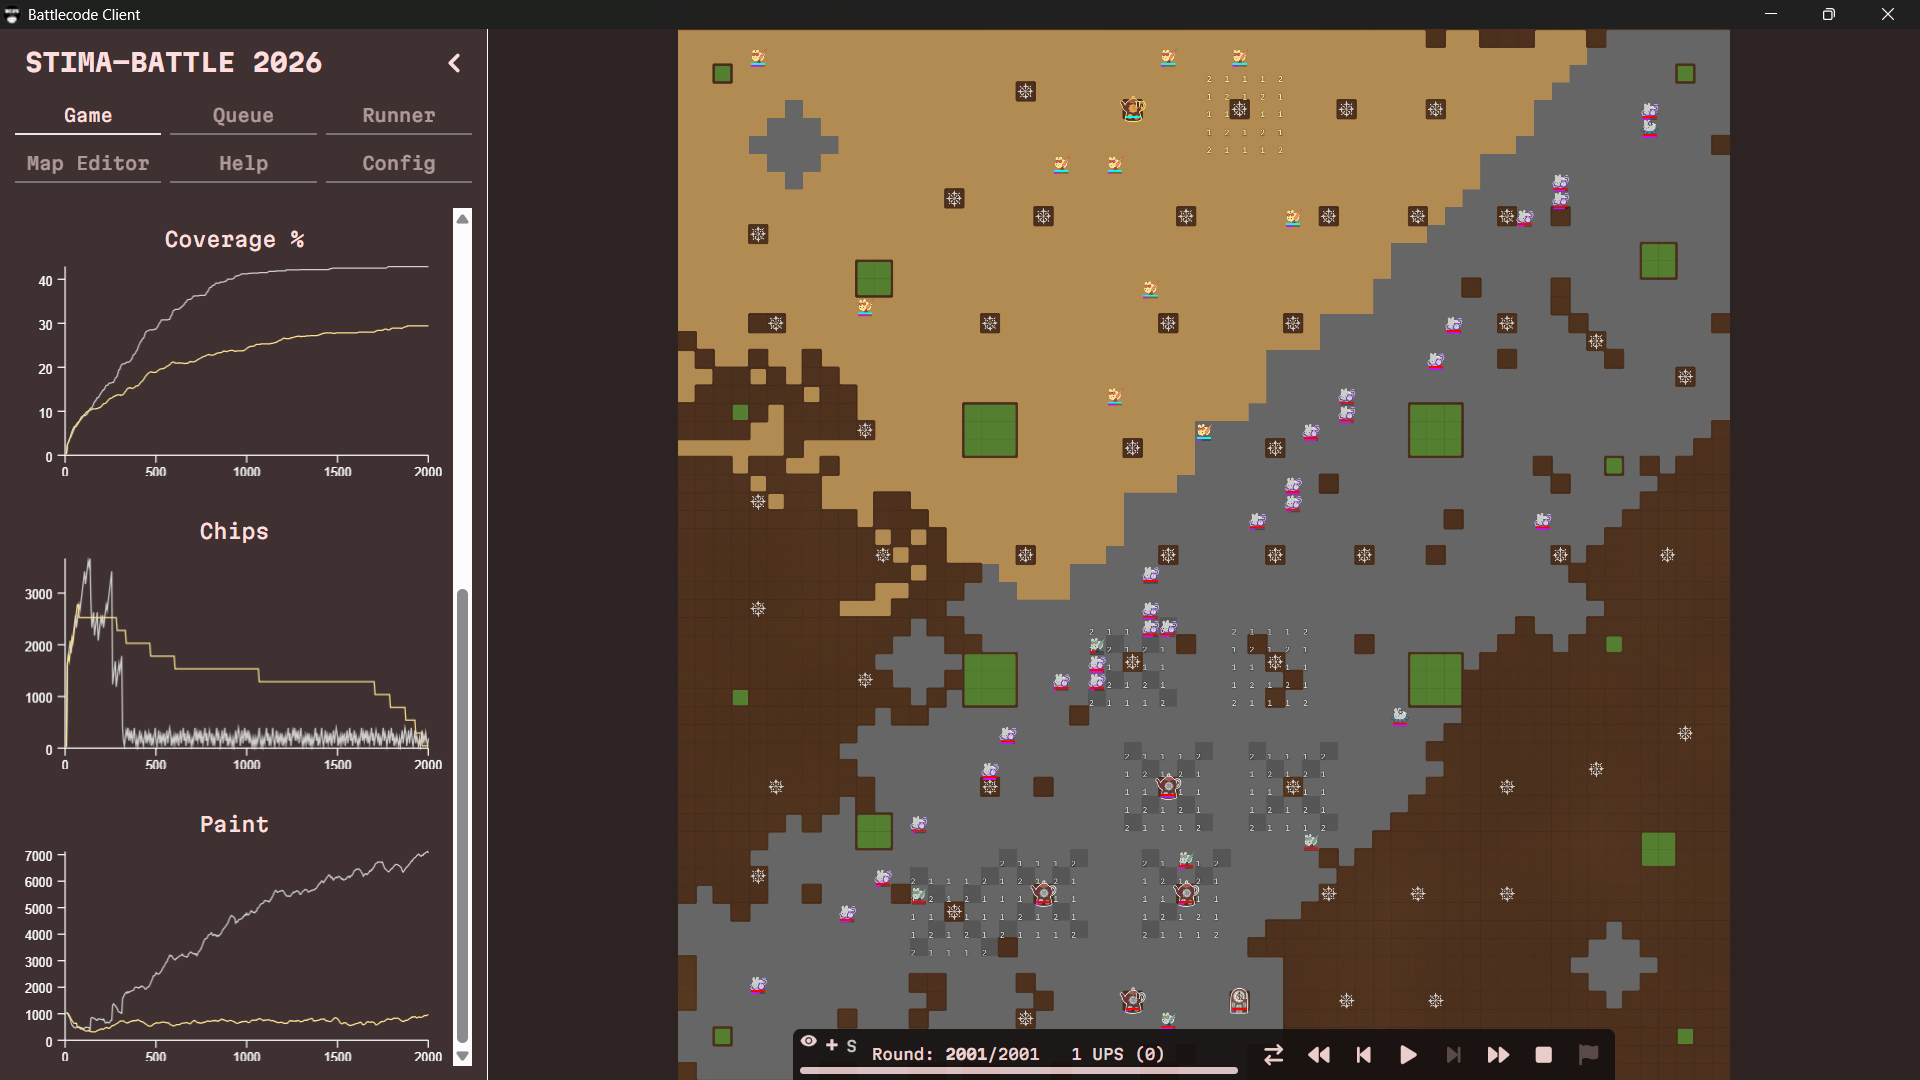
\includegraphics[width=0.5\textwidth]{images/mainbotvsaltbot1_huge.png}
    \caption{Statistik dan Kondisi Akhir mainbot vs altbot1 pada Map DefaultHuge}
    \label{fig:contoh}
\end{figure}

\subsubsection{mainbot vs altbot1 DefaultSmall (Pemenang : mainbot)}
\begin{figure}[H]
    \centering
    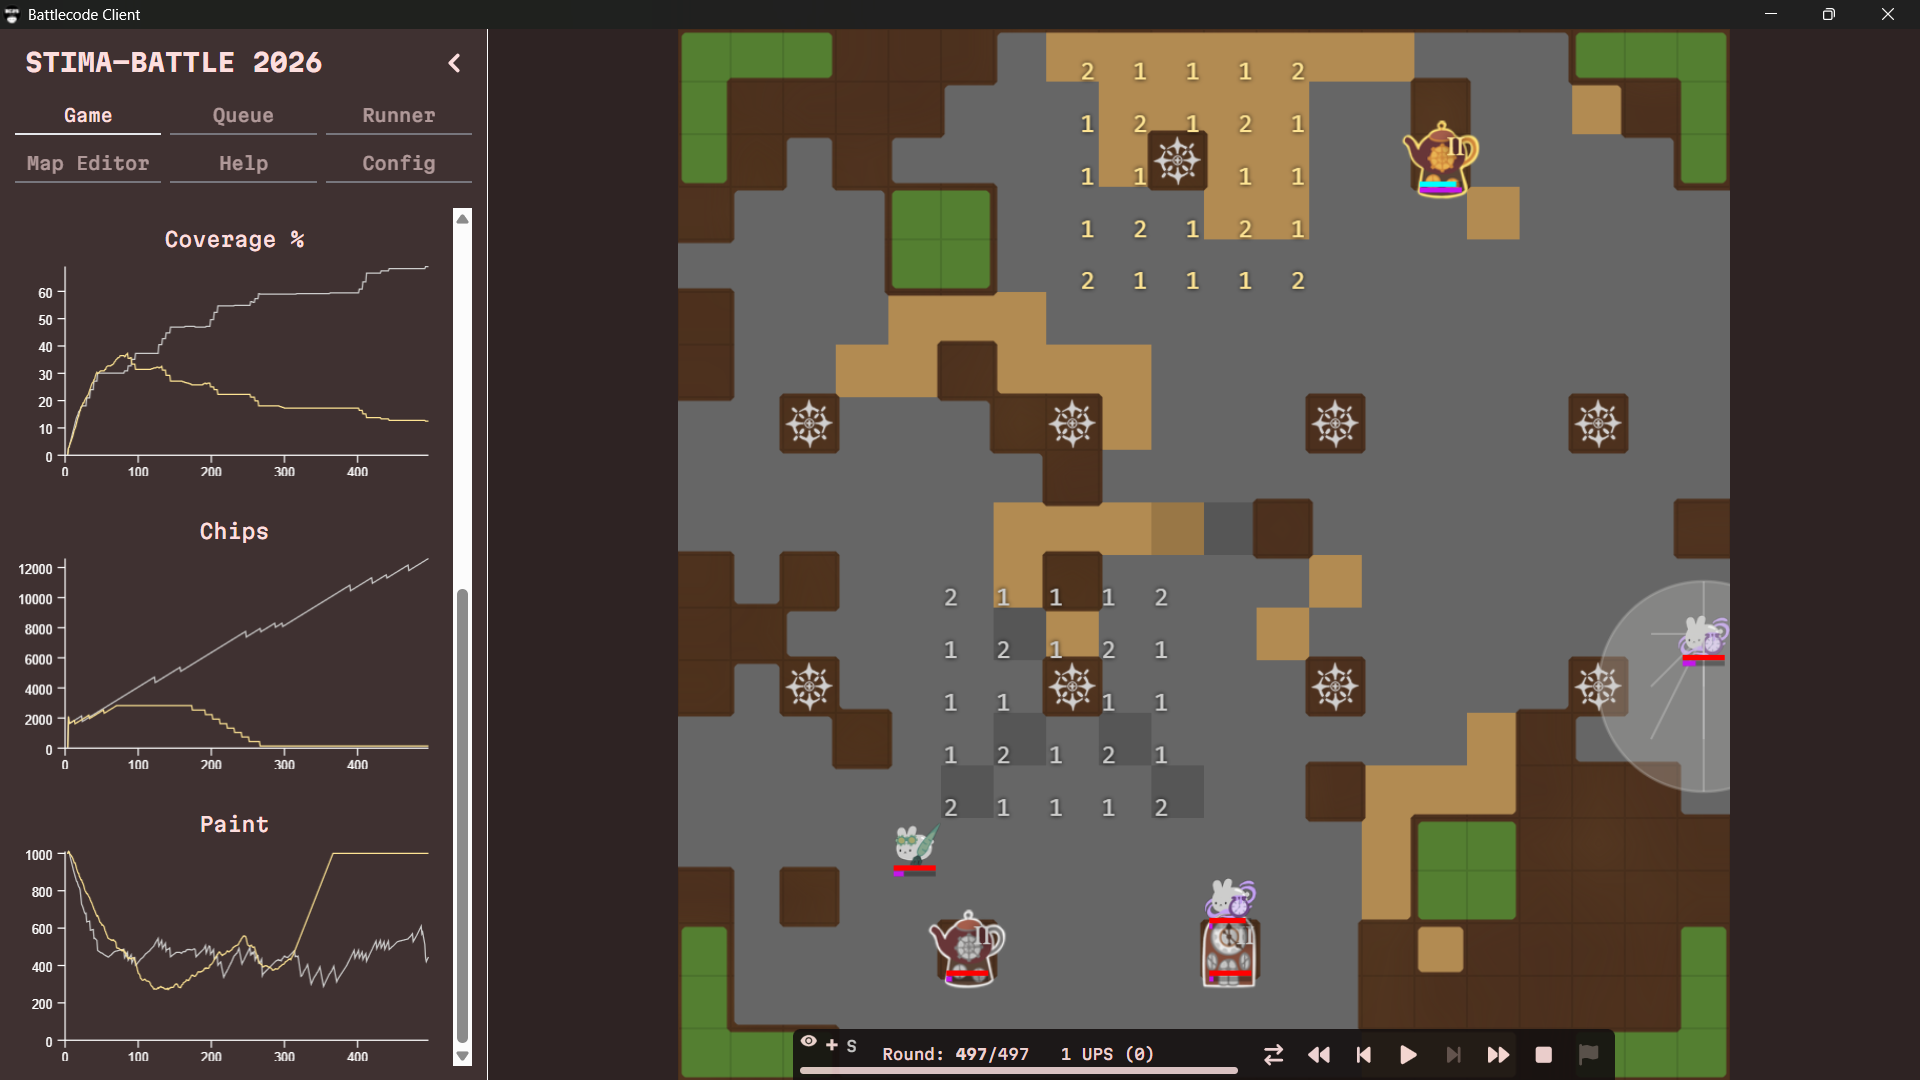
\includegraphics[width=0.5\textwidth]{images/mainbotvsaltbot1_small.png}
    \caption{Statistik dan Kondisi Akhir mainbot vs altbot1 pada Map DefaultSmall}
    \label{fig:contoh}
\end{figure}

\subsubsection{mainbot vs altbot1 DonkeyKong (Pemenang : mainbot)}
\begin{figure}[H]
    \centering
    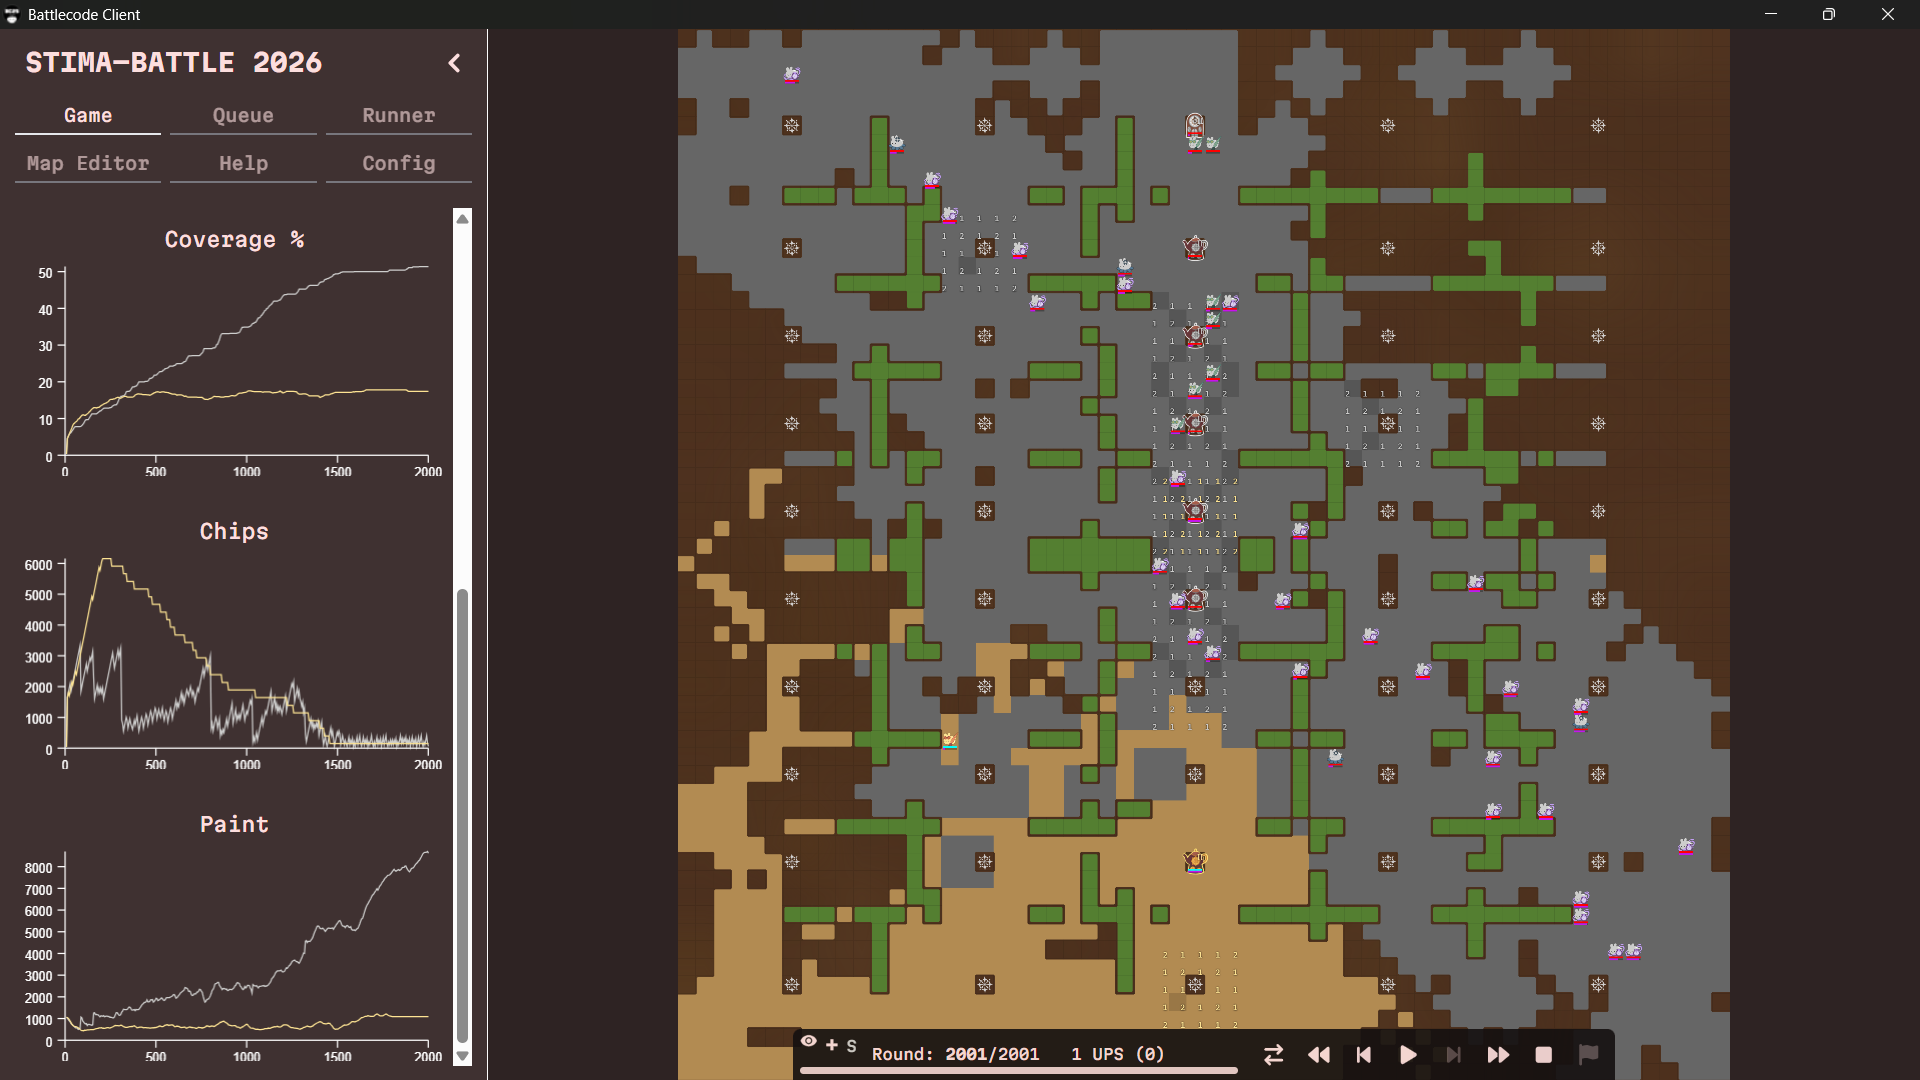
\includegraphics[width=0.5\textwidth]{images/mainbotvsaltbot1_donkey.png}
    \caption{Statistik dan Kondisi Akhir mainbot vs altbot1 pada Map DonkeyKong}
    \label{fig:contoh}
\end{figure}

\subsubsection{mainbot vs altbot2 DefaultHuge (Pemenang : mainbot)}
\begin{figure}[H]
    \centering
    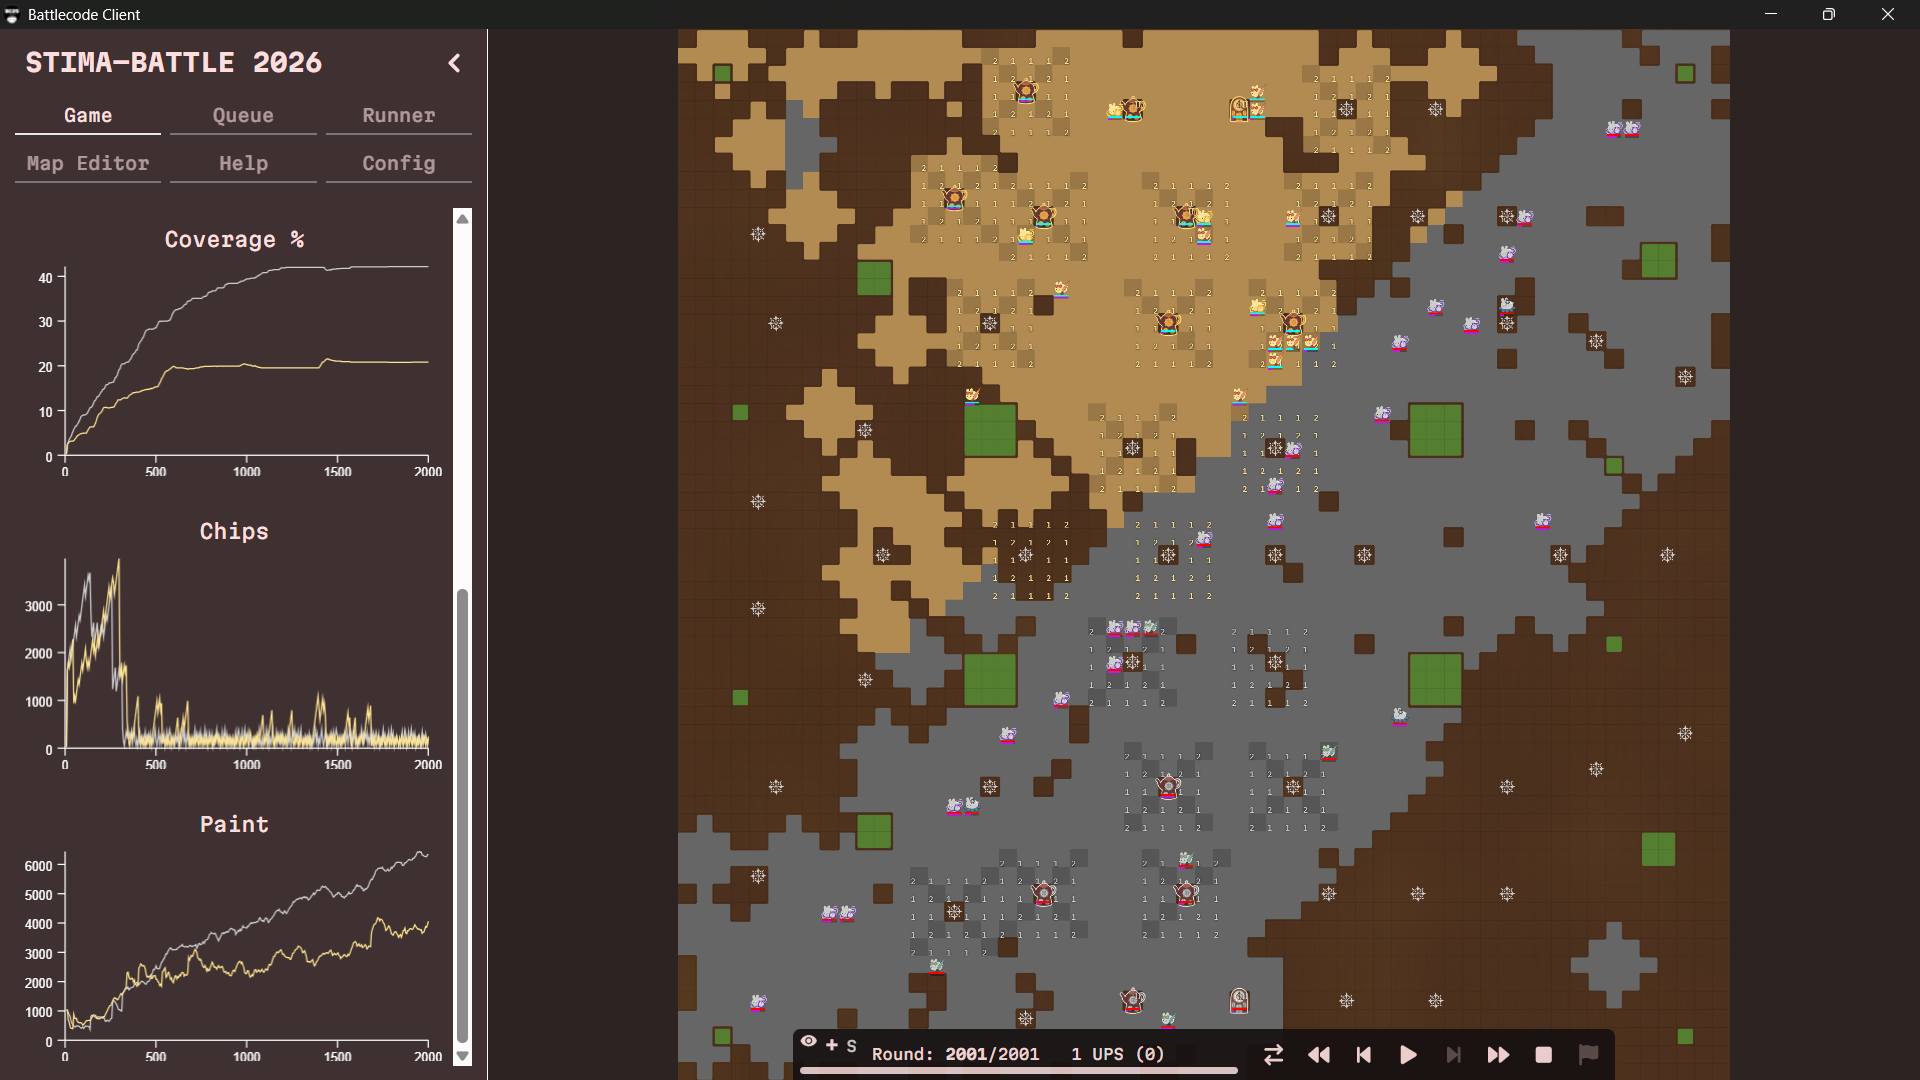
\includegraphics[width=0.5\textwidth]{images/mainbotvsaltbot2_huge.png}
    \caption{Statistik dan Kondisi Akhir mainbot vs altbot2 pada Map DefaultHuge}
    \label{fig:contoh}
\end{figure}

\subsubsection{mainbot vs altbot2 DefaultSmall (Pemenang : mainbot)}
\begin{figure}[H]
    \centering
    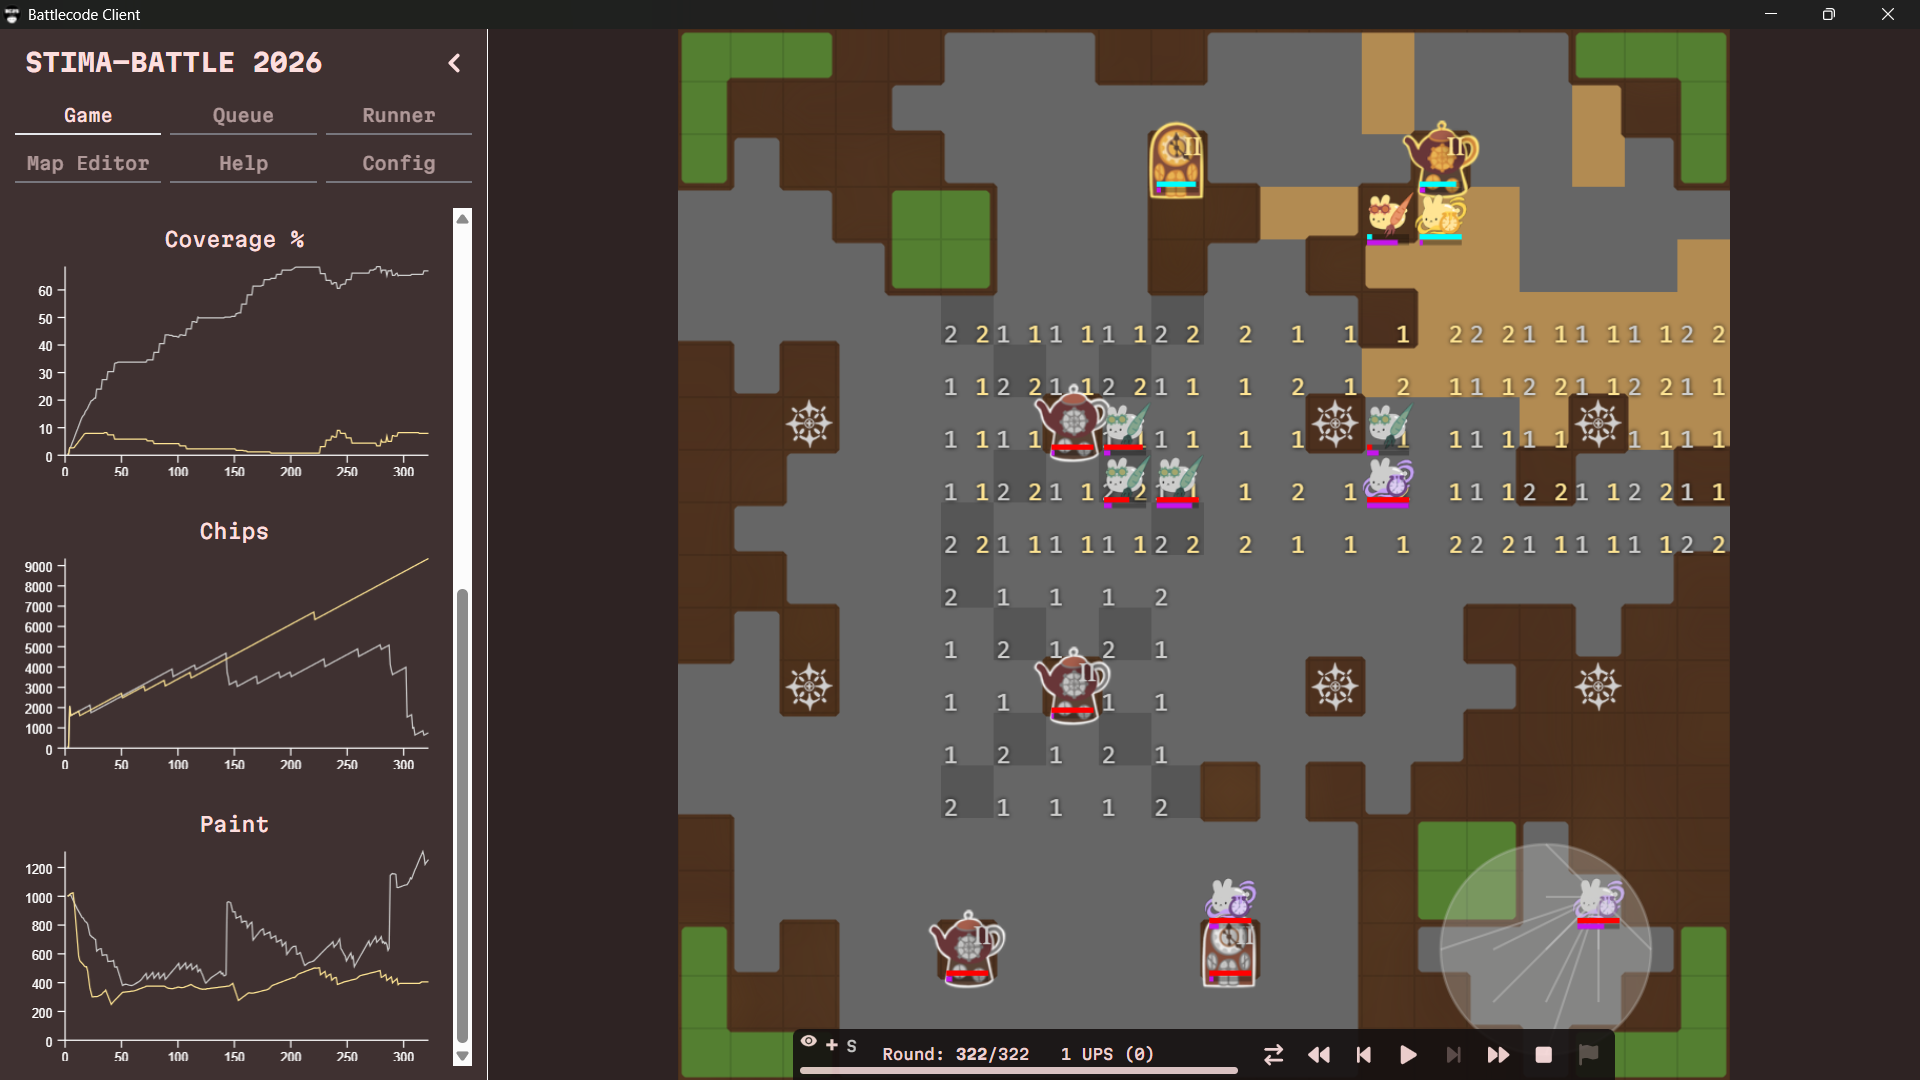
\includegraphics[width=0.5\textwidth]{images/mainbotvsaltbot2_small.png}
    \caption{Statistik dan Kondisi Akhir mainbot vs altbot2 pada Map DefaultSmall}
    \label{fig:contoh}
\end{figure}

\subsubsection{mainbot vs altbot2 DonkeyKong (Pemenang : mainbot)}
\begin{figure}[H]
    \centering
    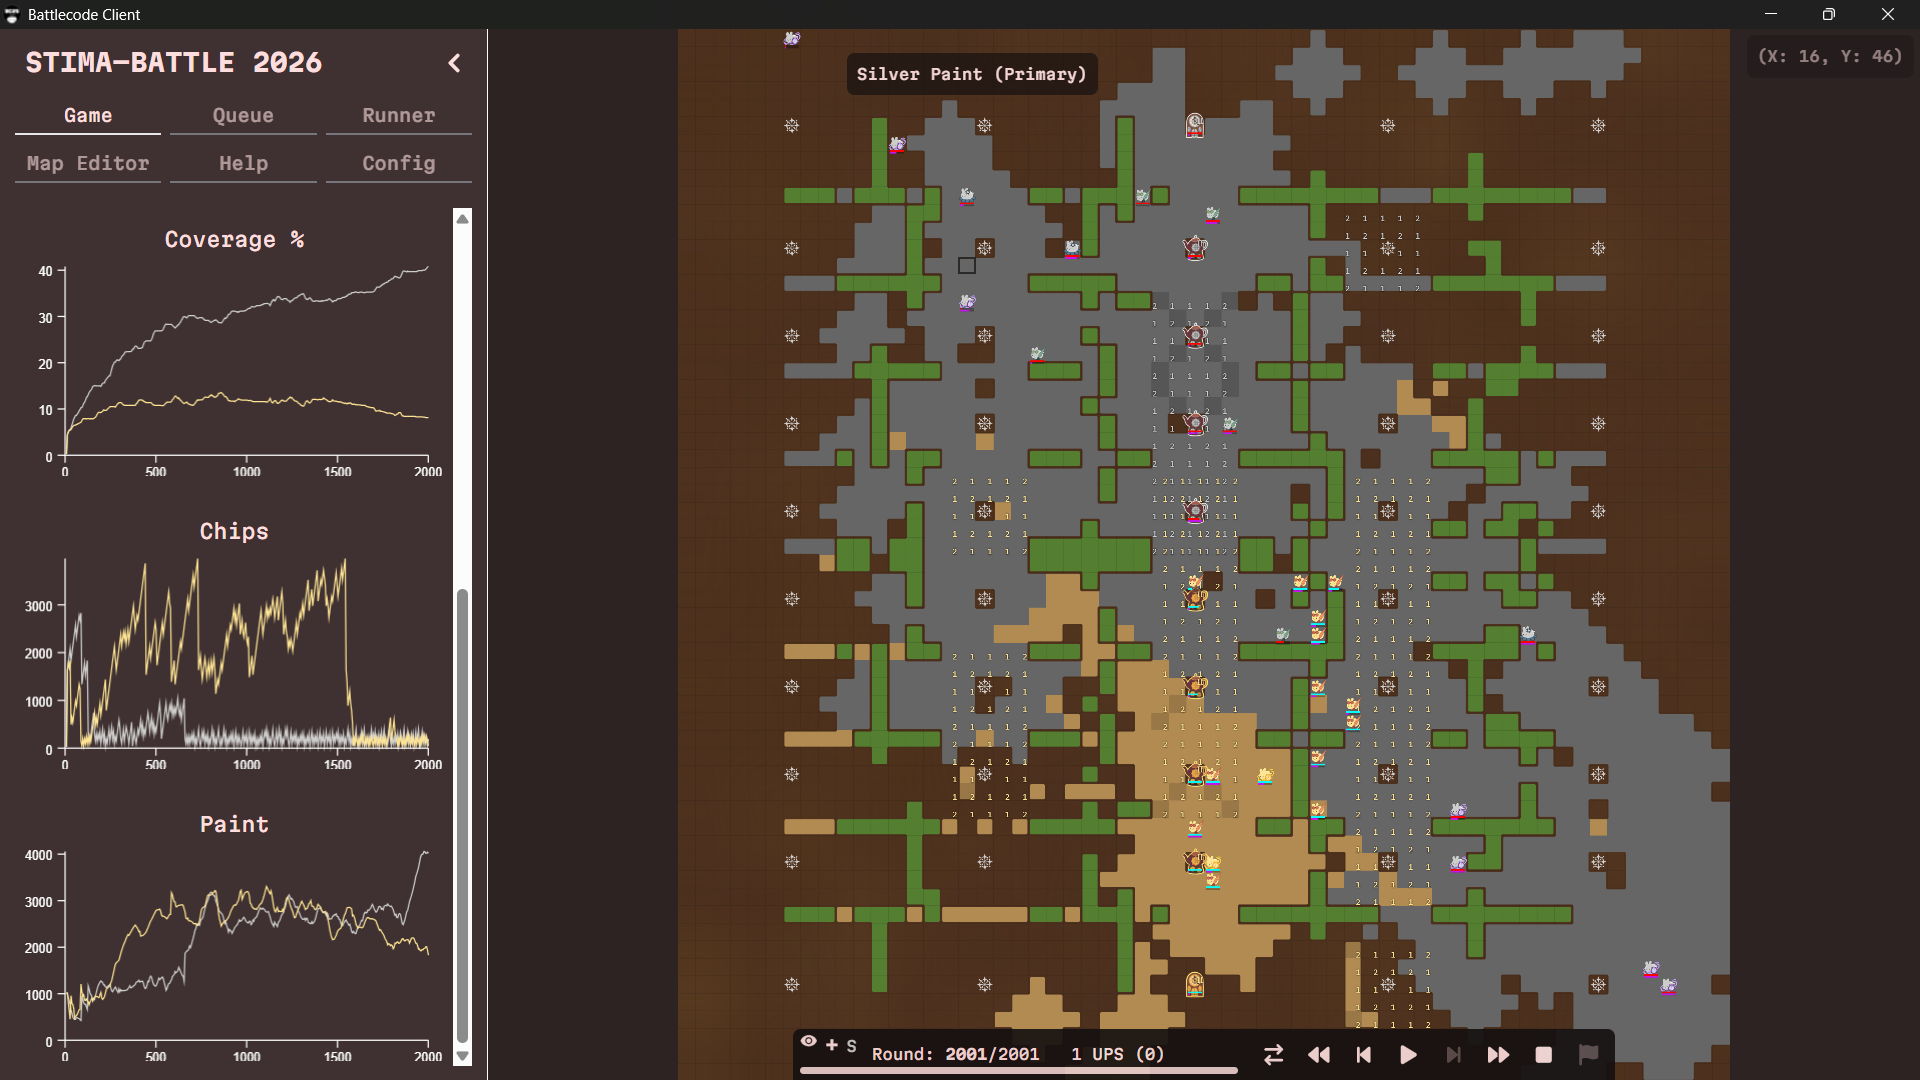
\includegraphics[width=0.5\textwidth]{images/mainbotvsaltbot2_donkey.png}
    \caption{Statistik dan Kondisi Akhir mainbot vs altbot2 pada Map DonkeyKong}
    \label{fig:contoh}
\end{figure}

\subsubsection{altbot1 vs altbot2 DefaultHuge (Pemenang : altbo1)}
\begin{figure}[H]
    \centering
    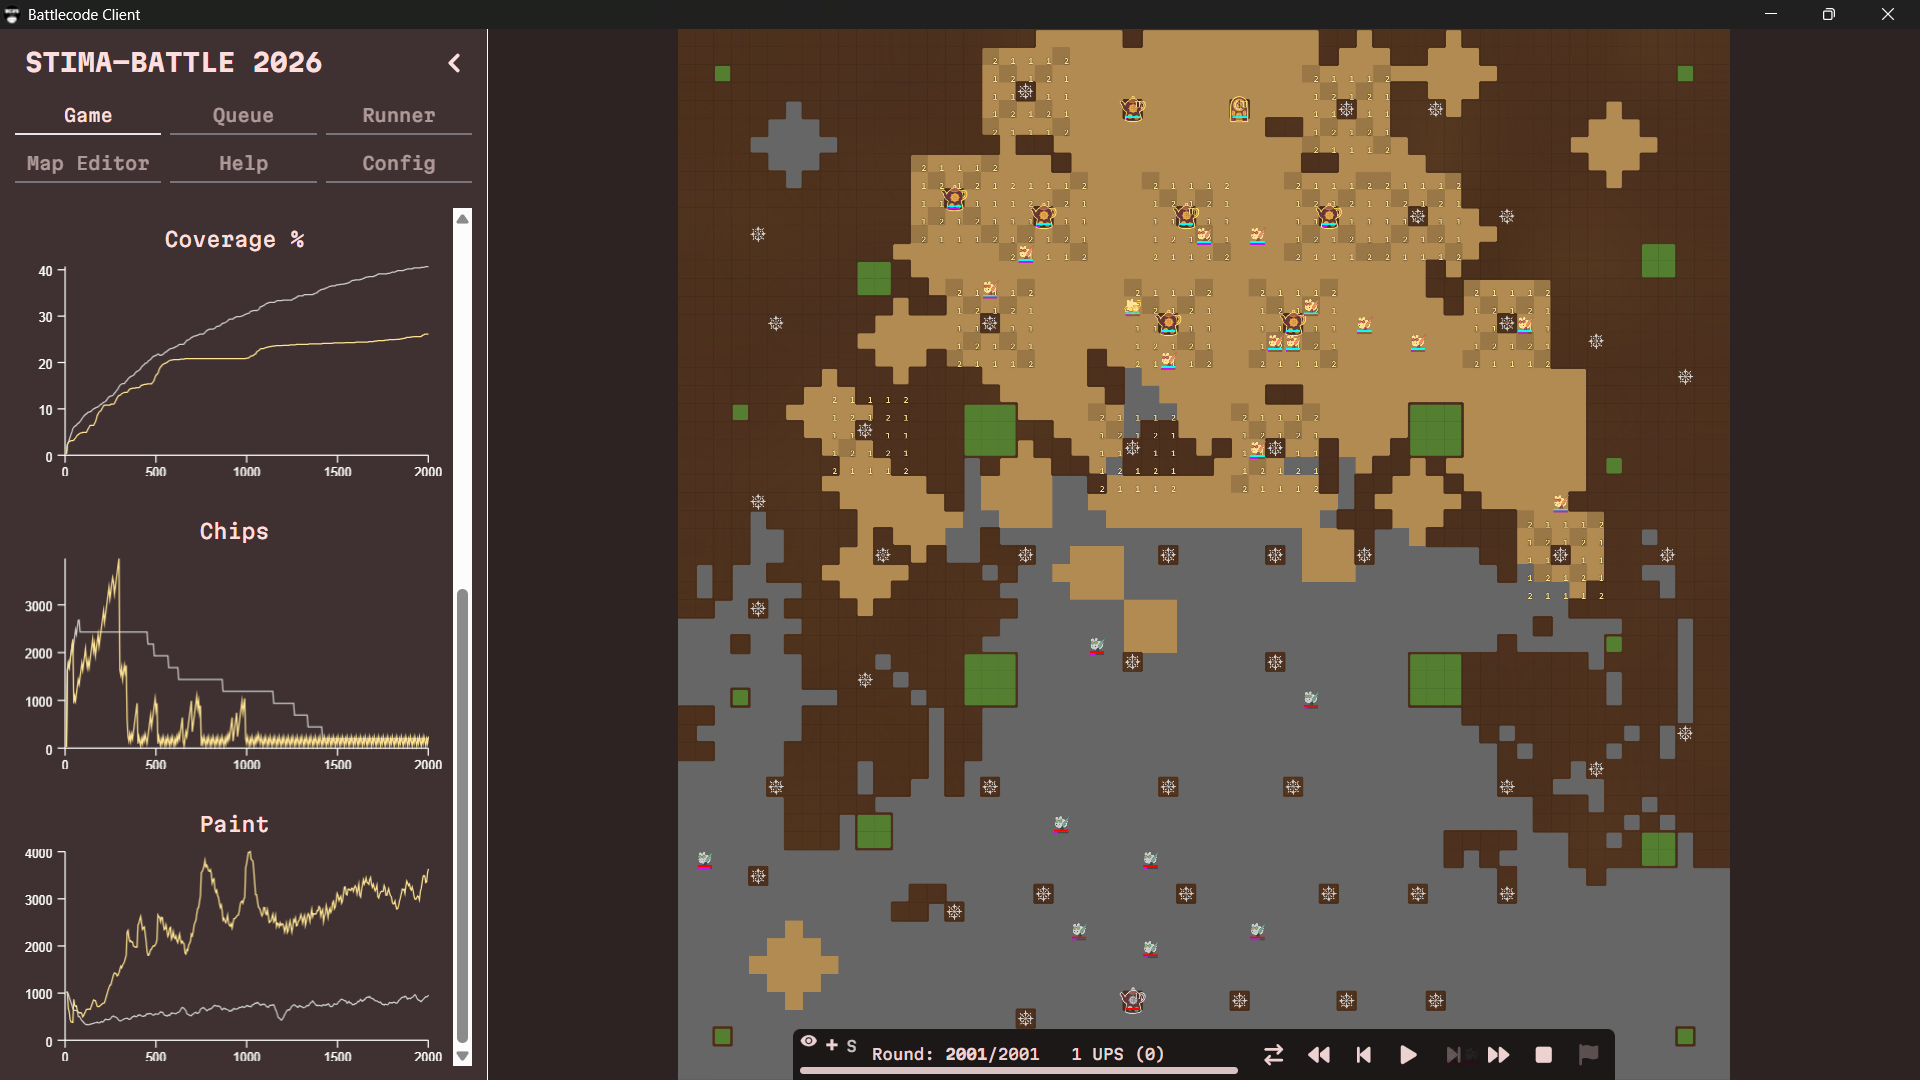
\includegraphics[width=0.5\textwidth]{images/altbot1vsaltbot2_huge.png}
    \caption{Statistik dan Kondisi Akhir altbot1 vs altbot2 pada Map DefaultHuge}
    \label{fig:contoh}
\end{figure}

\subsubsection{altbot1 vs altbot2 DefaultSmall (Pemenang : altbo2)}
\begin{figure}[H]
    \centering
    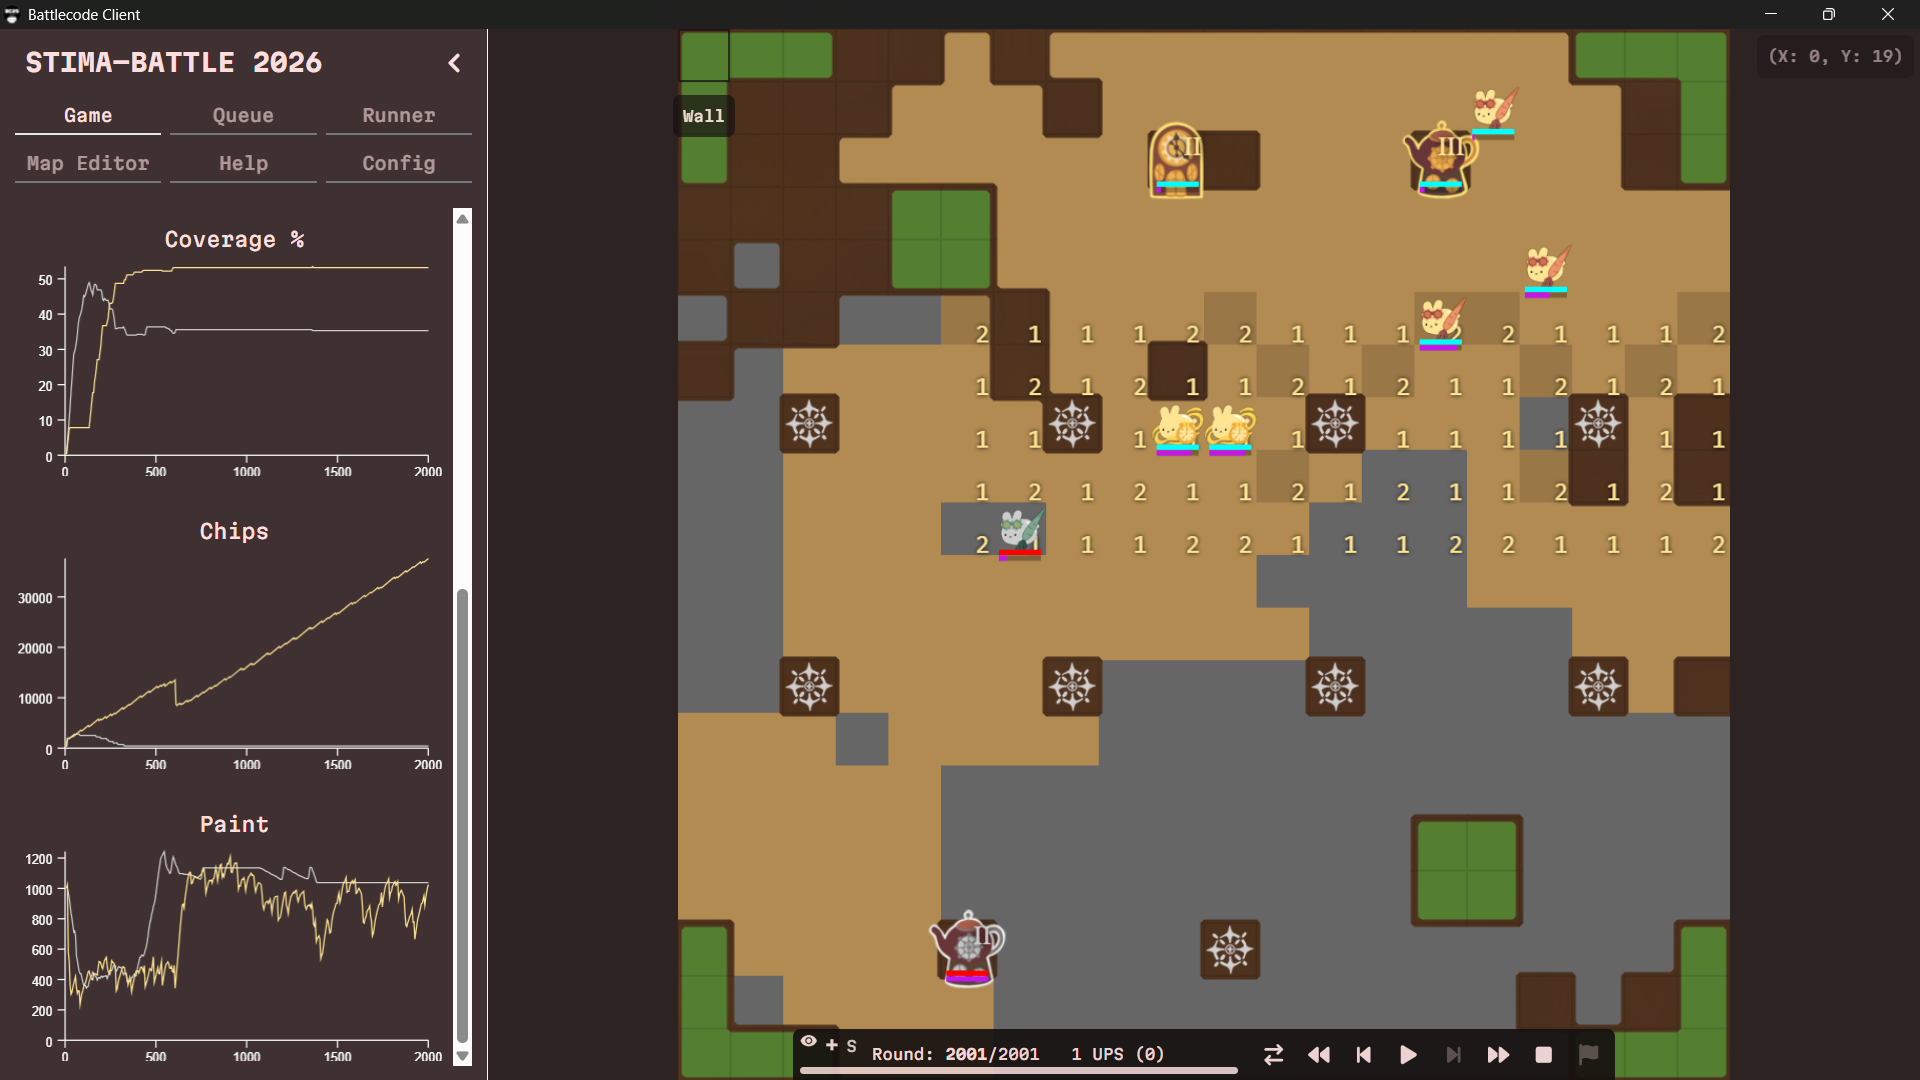
\includegraphics[width=0.5\textwidth]{images/altbot1vsaltbo2_small.png}
    \caption{Statistik dan Kondisi Akhir altbot1 vs altbot2 pada Map DefaultSmall}
    \label{fig:contoh}
\end{figure}

\subsubsection{altbot1 vs altbot2 DonkeyKong (Pemenang : altbo1)}
\begin{figure}[H]
    \centering
    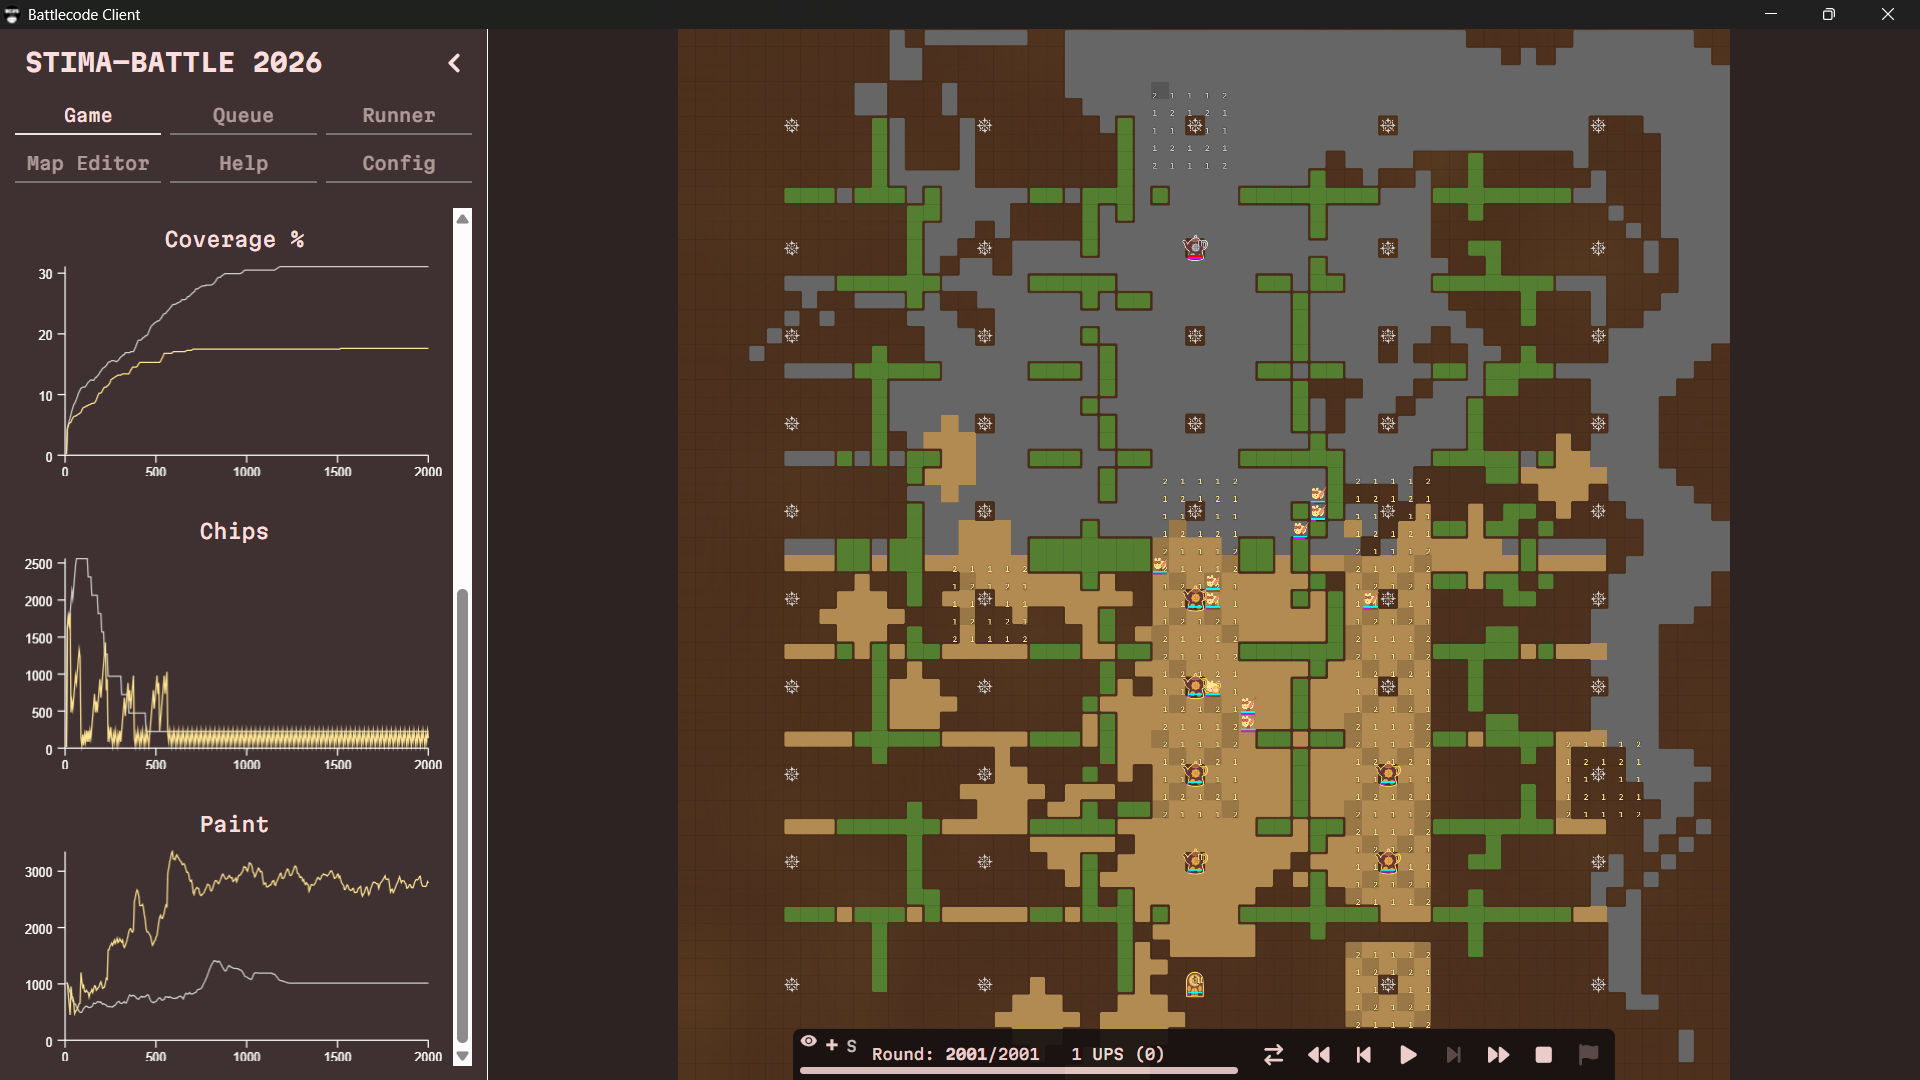
\includegraphics[width=0.5\textwidth]{images/altbot1vsaltbot2_donkey.png}
    \caption{Statistik dan Kondisi Akhir altbot1 vs altbot2 pada Map DonkeyKong}
    \label{fig:contoh}
\end{figure}

\subsection{Analisis Hasil Pengujian}